\documentclass[tikz,border=5pt]{standalone}
\usepackage{graphicx}
\usepackage{tikz}
\usetikzlibrary{arrows.meta, positioning, calc, shapes.geometric, fit}

\begin{document}

\begin{tikzpicture}[
  font=\sffamily,
  node distance=1.5cm and 1.8cm,
  >=Stealth,
  every node/.style={align=center}
]

% Input Image
\node (image) at (-6,0) {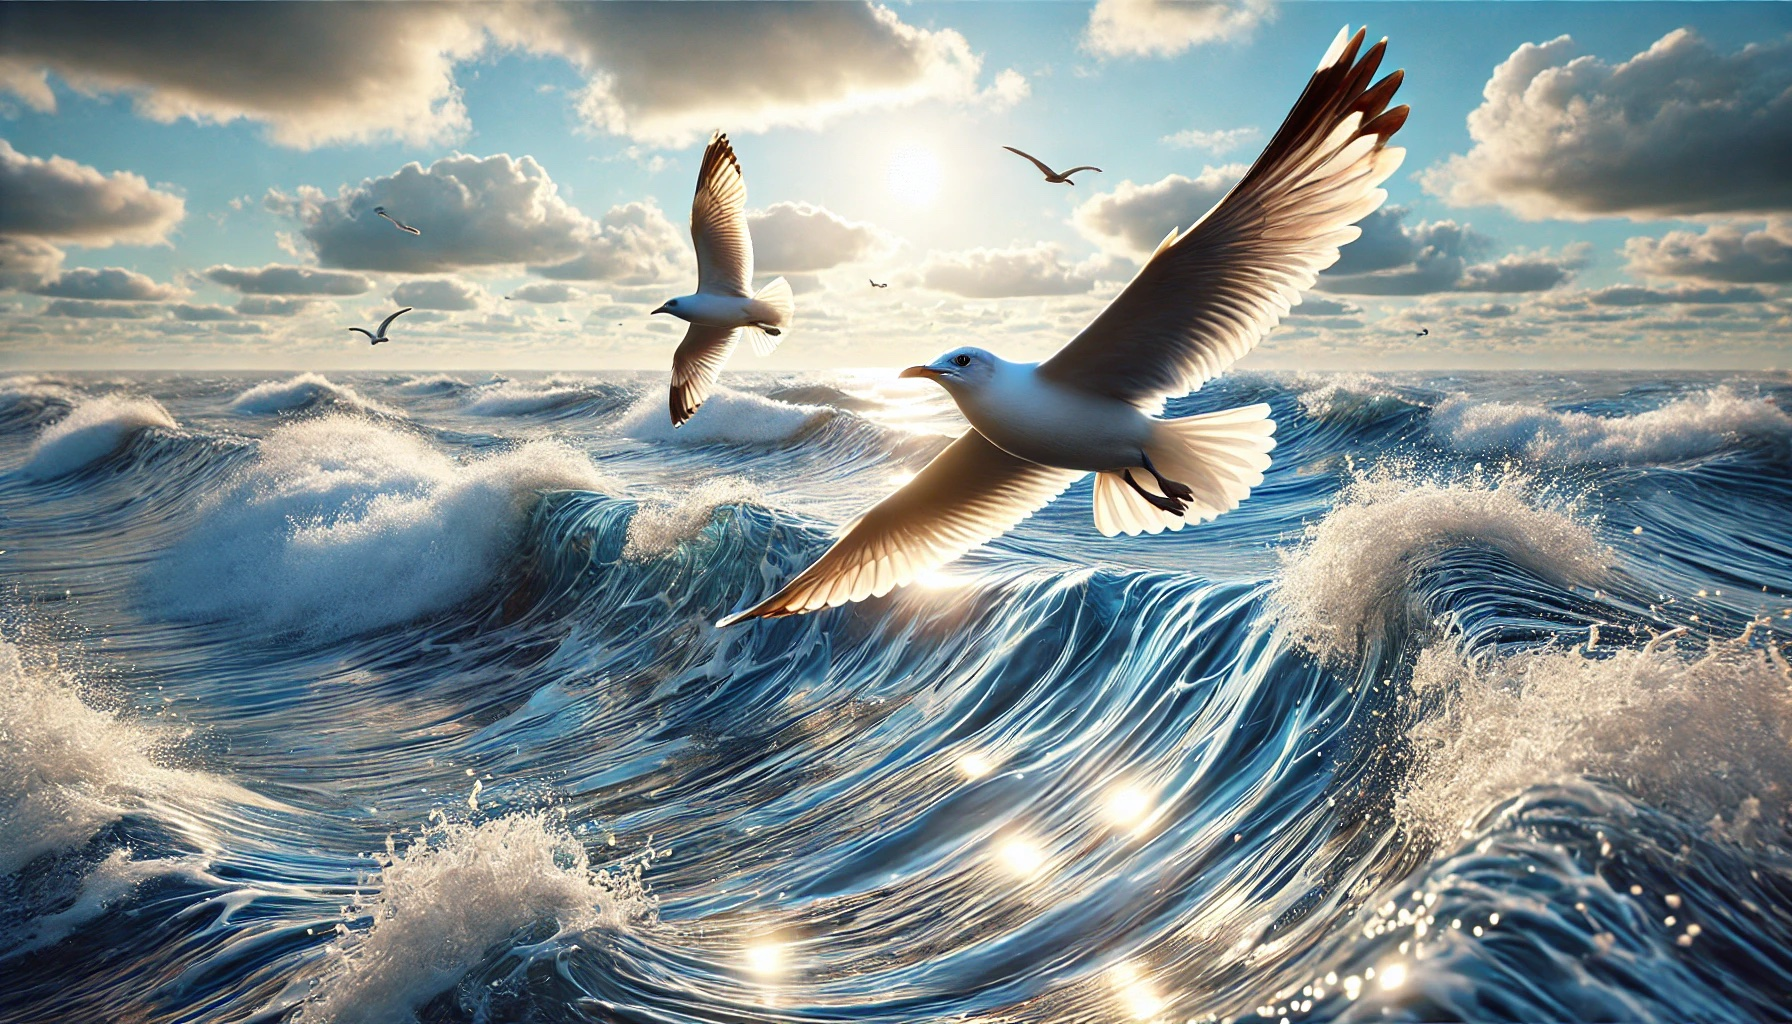
\includegraphics[width=2.5cm]{gulls.jpg}};

% Multi-scale feature pyramid
\node[draw, thick, rectangle, fill=blue!20, minimum width=1.5cm, minimum height=0.5cm] (level1) at (-1, 1.7) {};
\node[draw, thick, rectangle, fill=blue!40, minimum width=2cm, minimum height=0.7cm] (level2) at (-1, 1) {};
\node[draw, thick, rectangle, fill=blue!60, minimum width=2.5cm, minimum height=1cm] (level3) at (-1, 0) {};
\node[draw, thick, rectangle, fill=blue!80, minimum width=3cm, minimum height=1.3cm] (level4) at (-1, -1.3) {};

\node[left=0.3cm of level4] {High Resolution};
\node[left=0.3cm of level1] {Low Resolution};

% Arrows from image to pyramid levels
\foreach \i in {1,2,3,4} {
  \draw[->, thick] (image.east) -- (level\i.west);
}

% Flatten operation
\node[draw, thick, rectangle, fill=gray!30, minimum width=1.8cm, minimum height=0.8cm, right=of level3] (flatten) {Flatten \\ + Positional Embeddings};

\foreach \i in {1,2,3,4} {
  \draw[->, thick] (level\i.east) -- (flatten.west);
}

% Encoder block
\node[draw, thick, rectangle, fill=blue!30, minimum width=2.8cm, minimum height=1.2cm, right=of flatten] (encoder) {Encoder Layers \\ $\times N$};

% Query Selection
\node[draw, thick, rectangle, fill=gray!50, minimum width=2.5cm, minimum height=0.8cm, above=0.6cm of encoder] (query) {Query Selection};

% Arrows from flatten to encoder
\draw[->, thick] (flatten.east) -- (encoder.west);
\draw[->, thick] (encoder.north) -- (query.south);

% Decoder block
\node[draw, thick, rectangle, fill=gray!30, minimum width=2.8cm, minimum height=1.2cm, right=3.5cm of encoder] (decoder) {Decoder Layers \\ $\times M$};

% Arrows from encoder to decoder
\draw[->, thick] (encoder.east) -- node[above] {Keys \& Values} (decoder.west) ;

% Init Anchors and Noise
\node[draw, thick, rectangle, fill=yellow!40, minimum width=1.5cm, minimum height=0.8cm, right=1.0cm of query] (init) {Init Anchors};
\node[draw, thick, circle, fill=red!40, minimum width=0.5cm, below=2.5cm of init] (noise) {GT \\ + Noise};

% Arrows for noise and init anchors
\draw[->, thick] (init.south) -- (noise.north);
\draw[->, thick] (query.east) -- (init.west);
\draw[->, thick] (noise.east) -- (decoder.west);


% Matching and CDN
\node[draw, thick, rectangle, fill=gray!60, minimum width=2.5cm, minimum height=0.8cm, above=0.6cm of decoder] (matching) {Matching using\\ Contrastive \\ Denoising};

% Arrows from decoder to matching/CDN
\draw[->, thick] (decoder.north) -- (matching.south);



\end{tikzpicture}

\end{document}
